\chapter{Exploratory Study}
I am not positive I will include the results of my first study in the thesis, but this is a placeholder. Also, I might include a chapter about ``Patterns and Trends'' at large with reading level and topic on the Electome dataset, for the analysis I did on that.

This might morph into an ``additional data collection'' portion for the Twitter analysis.

% \section{Motivation}

% What was the purpose of the study?
% What were the hypotheses? 

% \section{Experimental Design} 

% \subsection{Dataset}
%     \subsubsection {Data Selection} 

%     For this study, we chose to analyze stories collected between January 1, 2016 (the start of the election year) and March 1, 2016 (Super Tuesday). Since a large number of states hold primary elections and caucuses on Super Tuesday, it is seen as an early indicator of candidate electability. All stories had been filtered through both the election (see section 3.3) and topic (see section 3.4) classifiers.

%     Based on the results of Super Tuesday, we selected four candidates for this study by delegate count: Hillary Clinton (1,279), Bernie Sanders (1,027), Donald Trump (743), and Ted Cruz (517) \cite{March45online}.

%     News articles were then separated into single-candidate stories (i.e. articles featuring primarily one candidate in the headline) to be able to measure more clearly the perceived bias per candidate. This was done programatically using regular expressions to determine if a headline contained one candidate and one candidate only. A dictionary of related names was created to make sure that stories were correctly categorized (i.e. ``Hillary'', ``Clinton'', and ``Hillary Clinton'' were to be categorized as pertaining to ``Hillary Clinton'' but not if preceded by ``Bill'').

%     \subsubsection {Publication Selection}

%     For the purposes of this study, stories were examined from five outlets: 

%     \begin{itemize}
%     \itemsep-1em 
%       \item CNN
%       \item Fox News  
%       \item The New York Times
%       \item The Wall Street Journal 
%       \item The Associated Press 
%     \end{itemize}

%     The choices consist of two pairs of outlets in both print and television across the liberal-conservative divide, plus a wire service. Of the 14 outlets above, both Fox News and the Wall Street Journal have an audience that leans conservative compared to the overall population (27\% mostly conservative viewers versus 17\% in the overall population for Fox News and 22\% mostly conservative viewers versus 17\% in the overall population) measured by a 2014 Pew survey \cite{PoliticalPolarization}.

%     On the other hand, the New York Times and CNN both have audiences that lean mostly liberal (25\% liberal versus 22\% in all respondents for CNN and 25\% for the New York Times). The Associated Press, which was not included in the survey, has members in outlets across the political divide and was chosen as an experimental control. 

%     [MIGHT INCLUDE THOSE DISTRIBUTIONS HERE]

%     \subsubsection{Topic Selection}

%     The top four topics by volume (Immigration, Abortion, Campaign Finance, Foreign Policy/National Security) were chosen for the survey to ensure a significant number of stories for each candidate for each topic. For overall topic distributions, see \ref{fig:topics} in the Appendix.
     

%     \subsubsection{Story Redaction}
%     For those readers in Group B (no disclosure of source), stories were further redacted to remove \emph{all mentions of news publications} in the body of the text and headline, to prevent readers from making assumptions about the source. The redacted words were replaced with the placeholder ``xxx'' and explained in the instructions for the task.


% \subsection{Survey} 







% \begin{figure}[h!] 
% \centering
%   \frame{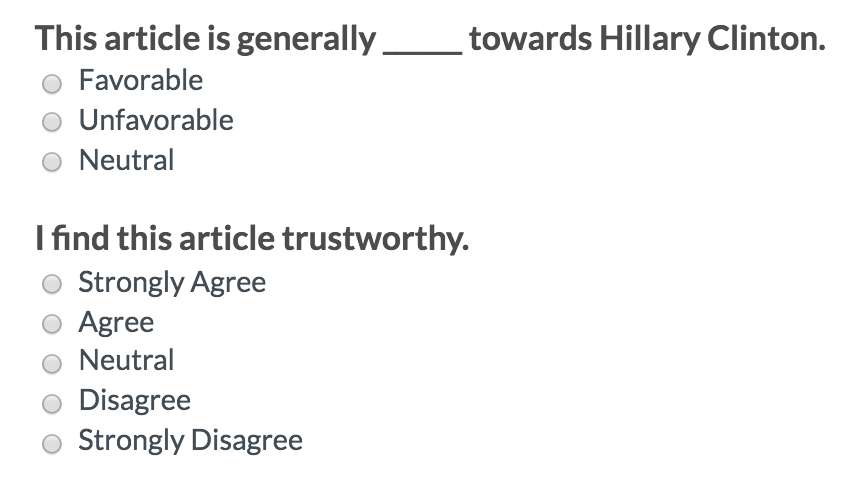
\includegraphics[width=0.45\textwidth]{study1_qs}}
%   \caption{Survey Questions for Study 1}
% \end{figure}








% \subsection{Quality Control}

% CrowdFlower has a built-in ``Test Question'' feature that allows for the rejection of a annotator whose answers to specific questions do not lie within a threshold (default 70\%) of the ``correct'' answer or whose answers lay outside the standard variation compared to others.

% However, since the questions we asked were by nature subjective and therefore outliers and disagreements in answers could imply signal rather than noise, we chose to monitor for quality using other metrics instead. CrowdFlower was not designed explicitly for survey-like tasks, and therefore there were no options for different screening methods or questions. Gold Questions on the platform are selected by the creator within the set of all questions being recorded.

% Because of this, we monitored quality of results in two ways:

% First, by setting a minimum of time of 180 seconds to complete the task of reading 5 stories for a task to be accepted,

% And second, by selecting only Level 3 contributors on CrowdFlower as suggested on their website for handling survey-like tasks \cite{CrowdFlower-guide}.

% Level 3 contributors are described as those who ``have completed over a hundred Test Questions across hundreds of different Job types, and have a near perfect overall Accuracy'' \cite{Crowdflower-levels}. This is the highest category of contributor.
 
% Users were also only allowed to answer the set of questions once. 

% Average response time was 07:31 minutes.
% \$0.50 was given per survey, as suggested by MIT Committee on the Use of Humans as Experimental Subjects \cite{COUHES-turk}.
% \section{Analysis}
% \section{Conclusions}

% \section{Limitations}

% From our exploratory study on reading level effects, we were able to obtain a significant but weak effect between disclosing the source and the levels of trust marked by readers towards an article.

% We also observed trends that suggested an interaction between disclosing the source and the reading level of a story.

% However, the study faced several limitations: first, we did not obtain enough samples to show a statistically significant result for interactions between source and reading level.

% Furthermore, multiple levels of independent variables (ie: 5 levels for input source) made modeling complex and the results less clear.

% The dataset was also unbalanced and sparse (ie, because of large numbers of input variables we did not have complete representation for each category, such as high, low, and mid-reading level stories for every outlet and topic). We tried to control for those factors by randomization, however it made more difficult to analyze specific correlations between source and trust.

% To further explore the interaction between disclosing the source and the reading level of the story, we set up another crowdsourcing experiment on CrowdFlower, this time targeting this specific interaction, to see if there is a significant effect between the two, detailed in the following chapter.